%\pdfminorversion=4
\documentclass[fleqn,aspectratio=169]{beamer}

% when making printed slides
\usepackage{pgfpages}
\pgfpagesuselayout{resize to}[a4paper,landscape,border shrink=5mm]

\usepackage[english]{babel}
\usepackage{tikz}
\usepackage{courier}
\usepackage{array}
\usepackage{bold-extra}
%\usepackage{minted}
\usepackage[thicklines]{cancel}
\usepackage{fancyvrb}
\usepackage{kotex}
\usepackage{paralist}
\usepackage{collectbox}
\usepackage{bm}

\usepackage{mathrsfs}
\usepackage[reqno,disallowspaces]{mathtools}  % imports amsmath
\usepackage{amsfonts} %for Y&Y BSR AMS fonts
\usepackage{amssymb}
\usepackage{amscd}
%\usepackage{tikz,lipsum,lmodern}
\usepackage[most]{tcolorbox}
\usepackage{verbatim}
\mode<presentation>
{
  \usetheme{default}
  \usecolortheme{default}
  \usefonttheme{default}
  \setbeamertemplate{navigation symbols}{}
  \setbeamertemplate{caption}[numbered]
  \setbeamertemplate{footline}[frame number]  % or "page number"
  \setbeamercolor{frametitle}{fg=yellow}
  \setbeamercolor{footline}{fg=black}
} 

\setbeamercolor{block body alerted}{bg=alerted text.fg!10}
\setbeamercolor{block title alerted}{bg=alerted text.fg!20}
\setbeamercolor{block body}{bg=structure!10}
\setbeamercolor{block title}{bg=structure!20}
\setbeamercolor{block body example}{bg=green!10}
\setbeamercolor{block title example}{bg=green!20}
\setbeamertemplate{blocks}[rounded][shadow]

\xdefinecolor{dianablue}{rgb}{0.18,0.24,0.31}
\xdefinecolor{darkblue}{rgb}{0.1,0.1,0.7}
\xdefinecolor{darkgreen}{rgb}{0,0.5,0}
\xdefinecolor{darkgrey}{rgb}{0.35,0.35,0.35}
\xdefinecolor{darkorange}{rgb}{0.8,0.5,0}
\xdefinecolor{darkred}{rgb}{0.7,0,0}
\definecolor{darkgreen}{rgb}{0,0.6,0}
\definecolor{mauve}{rgb}{0.58,0,0.82}

\usetikzlibrary{shapes.callouts}

\makeatletter
\setbeamertemplate{footline}
{
  \leavevmode%
  \hbox{%
  \begin{beamercolorbox}[wd=.333333\paperwidth,ht=2.25ex,dp=1ex,center]{author in head/foot}%
    \usebeamerfont{author in head/foot}\insertsection
  \end{beamercolorbox}%
  \begin{beamercolorbox}[wd=.333333\paperwidth,ht=2.25ex,dp=1ex,center]{title in head/foot}%
    \usebeamerfont{title in head/foot}\insertsubsection
  \end{beamercolorbox}%
  \begin{beamercolorbox}[wd=.333333\paperwidth,ht=2.25ex,dp=1ex,right]{date in head/foot}%
    \usebeamerfont{date in head/foot}
    \insertshortdate{}\hspace*{2em}
    \insertframenumber{} / \inserttotalframenumber\hspace*{2ex} 
  \end{beamercolorbox}}%

  \vskip0pt%
}
\makeatother



\title[]{Lecture 5: Vector Calculus}
\author{Yi, Yung (이융)}
\institute{Mathematics for Machine Learning\\ KAIST EE}
\date{MONTH DAY, 2021}

%%%%%%%%%%%% real, integer notation
\newcommand{\real}{{\mathbb R}}
\newcommand{\realn}{{\mathbb R}^{n}}
\newcommand{\realm}{{\mathbb R}^{m}}
\newcommand{\realD}{{\mathbb R}^{D}}
\newcommand{\realM}{{\mathbb R}^{M}}
\newcommand{\realN}{{\mathbb R}^{N}}
\newcommand{\realnn}{{\mathbb R}^{n \times n}}
\newcommand{\realmm}{{\mathbb R}^{m \times m}}
\newcommand{\realmn}{{\mathbb R}^{m \times n}}
\newcommand{\realnm}{{\mathbb R}^{n \times m}}
\newcommand{\realDM}{{\mathbb R}^{D \times M}}
\newcommand{\realMD}{{\mathbb R}^{M \times D}}
\newcommand{\complex}{{\mathbb C}}
\newcommand{\integer}{{\mathbb Z}}
\newcommand{\natu}{{\mathbb N}}


%%% set, vector, matrix
\newcommand{\set}[1]{\ensuremath{\mathcal #1}}
\newcommand{\sets}[1]{\ensuremath{\{#1 \}}}
\renewcommand{\vec}[1]{\bm{#1}}
\newcommand{\mat}[1]{\bm{#1}}

%%%% vector
\def\vx{\vec{x}}
\def\vy{\vec{y}}
\def\vz{\vec{z}}
\def\vf{\vec{f}}
\def\ve{\vec{e}}
\def\vr{\vec{r}}
\def\vb{\vec{b}}
\def\vc{\vec{c}}
\def\vd{\vec{d}}
\def\vm{\vec{m}}
\def\vu{\vec{u}}
\def\vv{\vec{v}}
\def\vw{\vec{w}}
\def\vX{\vec{X}}
\def\vY{\vec{Y}}
\def\vZ{\vec{Z}}
\def\vth{\vec{\theta}}
\def\vmu{\vec{\mu}}
\def\vnu{\vec{\nu}}
\def\vlam{\vec{\lambda}}
\def\vep{\vec{\epsilon}}
\def\vpi{\vec{\pi}}
\def\vphi{\vec{\phi}}
\def\vxi{\vec{\xi}}
\def\valpha{\vec{\alpha}}
\def\vgamma{\vec{\gamma}}

%%%% Well-used matrices
\def\mA{\mat{A}}
\def\mB{\mat{B}}
\def\mC{\mat{C}}
\def\mD{\mat{D}}
\def\mI{\mat{I}}
\def\mJ{\mat{J}}
\def\mK{\mat{K}}
\def\mE{\mat{E}}
\def\mP{\mat{P}}
\def\mQ{\mat{Q}}
\def\mU{\mat{U}}
\def\mV{\mat{V}}
\def\mR{\mat{R}}
\def\mS{\mat{S}}
\def\mX{\mat{X}}
\def\msig{\mat{\Sigma}}
\def\mPhi{\mat{\Phi}}


%%%%% vector caculus useful macro
% ...\d, which typesets a derivative. ex: \d{y}{x}, instead of \frac{dx}{dy}.
\renewcommand{\d}[2]{\frac{\text{d} #1}{\text{d} #2}}

% ...similar for double-derivatives. ex: \dd{y}{x}.
\newcommand{\dd}[2]{\frac{\text{d}^2 #1}{\text{d} #2^2}}

% ...similar for partial derivatives. ex: \pd{y}{x}.
\newcommand{\pd}[2]{\frac{\partial #1}{\partial #2}}

% ...similar for partial double derivatives. ex: \pdd{y}{x}.
\newcommand{\pdd}[2]{\frac{\partial^2 #1}{\partial #2^2}}
% pdd with argument
\newcommand{\pdda}[3]{\frac{\partial^2 #1}{\partial #2 \partial #3}}

\usepackage{xparse}

%%%% caligraphic fonts
\def\cL{\ensuremath{{\cal L}}}
\def\cN{\ensuremath{{\cal N}}}
\def\cD{\ensuremath{{\cal D}}}
\def\cC{\ensuremath{{\cal C}}}
\def\cX{\ensuremath{{\cal X}}}
\def\cY{\ensuremath{{\cal Y}}}

%%% big parenthesis
\def\Bl{\Bigl}
\def\Br{\Bigr}
\def\lf{\left}
\def\ri{\right}


%%% floor notations
\newcommand{\lfl}{{\lfloor}}
\newcommand{\rfl}{{\rfloor}}
\newcommand{\floor}[1]{{\lfloor #1 \rfloor}}

%%% gradient
\newcommand{\grad}[1]{\nabla #1}
\newcommand{\hess}[1]{\text{H} #1}

%%% definition
%\newcommand{\eqdef}{\ensuremath{\triangleq}}
\newcommand{\eqdef}{\ensuremath{:=}}
%%% imply
\newcommand{\imp}{\Longrightarrow}



\newcommand{\separator}{
%  \begin{center}
    \par\noindent\rule{\columnwidth}{0.3mm}
%  \end{center}
}

\newcommand{\mynote}[1]{{\it \color{red} [#1]}}







%%% equation alignment
\newcommand{\aleq}[1]{\begin{align*}#1\end{align*}}

%%%%%%%%%%%%%%%% colored emphasized font, blanked words

\newcommand{\empr}[1]{{\color{red}\emph{#1}}}
\newcommand{\empb}[1]{{\color{blue}\emph{#1}}}
\newcommand{\redf}[1]{{\color{red} #1}}
\newcommand{\bluef}[1]{{\color{blue} #1}}
\newcommand{\grayf}[1]{{\color{gray} #1}}
\newcommand{\magenf}[1]{{\color{magenta} #1}}
\newcommand{\greenf}[1]{{\color{green} #1}}
\newcommand{\cyanf}[1]{{\color{cyan} #1}}
\newcommand{\orangef}[1]{{\color{orange} #1}}

\newcommand{\blk}[1]{\underline{\mbox{\hspace{#1}}}}


\newcommand{\redblk}[1]{\framebox{\color{red} #1}}
\newcommand{\redblank}[2]{\framebox{\onslide<#1->{\color{red} #2}}}
\newcommand{\blueblk}[1]{\framebox{\color{blue} #1}}
\newcommand{\blueblank}[2]{\framebox{\onslide<#1->{\color{blue} #2}}}



\makeatletter
\newcommand{\mybox}{%
    \collectbox{%
        \setlength{\fboxsep}{1pt}%
        \fbox{\BOXCONTENT}%
    }%
}
\makeatother

\makeatletter
\newcommand{\lecturemark}{%
    \collectbox{%
        \setlength{\fboxsep}{1pt}%
        \fcolorbox{red}{yellow}{\BOXCONTENT}%
    }%
}
\makeatother

\newcommand{\mycolorbox}[1]{
\begin{tcolorbox}[colback=red!5!white,colframe=red!75!black]
#1
\end{tcolorbox}
}
%%%% figure inclusion
\newcommand{\mypic}[2]{
\begin{center}
\includegraphics[width=#1\textwidth]{#2}
\end{center}
}

\newcommand{\myinlinepic}[2]{
\makebox[0cm][r]{\raisebox{-4ex}{\includegraphics[height=#1]{#2}}}
}




%%%% itemized and enumerated list
\newcommand{\bci}{\begin{compactitem}}
\newcommand{\eci}{\end{compactitem}}
\newcommand{\bce}{\begin{compactenum}}
\newcommand{\ece}{\end{compactenum}}


%%%% making 0.5/0.5 two columns
%%%% how to use: first number: length of separation bar
% \mytwocols{0.6}
% {
% contents in the left column
% }
% {
% contents in the right column
% }
%%%%

\newcommand{\mytwocols}[3]{
\begin{columns}[T] \column{.499\textwidth} #2 \column{.001\textwidth} \rule{.3mm}{{#1}\textheight} \column{.499\textwidth} #3 \end{columns}}

\newcommand{\mythreecols}[4]{
\begin{columns}[T] \column{.31\textwidth} #2 \column{.001\textwidth} \rule{.3mm}{{#1}\textheight} \column{.31\textwidth} #3 \column{.001\textwidth} \rule{.3mm}{{#1}\textheight} \column{.31\textwidth} #4  \end{columns}}

\newcommand{\mysmalltwocols}[3]{
\begin{columns}[T] \column{.4\textwidth} #2 \column{.001\textwidth} \rule{.3mm}{{#1}\textheight} \column{.4\textwidth} #3 \end{columns}}

%%%% making two columns with customized ratios
%%%% how to use: 
%first parameter: length of separation bar
%second parameter: ratio of left column
%third parameter: ratio of right column
% \mytwocols{0.6}{0.7}{0.29}
% {
% contents in the left column
% }
% {
% contents in the right column
% }
%%%%
\newcommand{\myvartwocols}[5]{
\begin{columns}[T] \column{#2\textwidth} {#4} \column{.01\textwidth} \rule{.3mm}{{#1}\textheight} \column{#3\textwidth} {#5} \end{columns}}

%%% making my block in beamer
%%% first parameter: title of block
%%% second parameter: contents of block
\newcommand{\myblock}[2]{
\begin{block}{#1} {#2}  \end{block}}

%%% independence notation
\newcommand{\indep}{\perp \!\!\! \perp}

%%%% probability with different shapes (parenthesis or bracket) and different sizes
%%% `i' enables us to insert the subscript to the probability 
\newcommand{\bprob}[1]{\mathbb{P}\Bl[ #1 \Br]}
\newcommand{\prob}[1]{\mathbb{P}[ #1 ]}
\newcommand{\cbprob}[1]{\mathbb{P}\Bl( #1 \Br)}
\newcommand{\cprob}[1]{\mathbb{P}( #1 )}
\newcommand{\probi}[2]{\mathbb{P}_{#1}[ #2 ]}
\newcommand{\bprobi}[2]{\mathbb{P}_{#1}\Bl[ #2 \Br]}
\newcommand{\cprobi}[2]{\mathbb{P}_{#1}( #2 )}
\newcommand{\cbprobi}[2]{\mathbb{P}_{#1}\Bl( #2 \Br)}

%%%% expectation with different shapes (parenthesis or bracket) and different sizes
%%% `i' enables us to insert the subscript to the expectation
\newcommand{\expect}[1]{\mathbb{E}[ #1 ]}
\newcommand{\cexpect}[1]{\mathbb{E}( #1 )}
\newcommand{\bexpect}[1]{\mathbb{E}\Bl[ #1 \Br]}
\newcommand{\cbexpect}[1]{\mathbb{E}\Bl( #1 \Br)}
\newcommand{\bbexpect}[1]{\mathbb{E}\lf[ #1 \ri]}
\newcommand{\expecti}[2]{\mathbb{E}_{#1}[ #2 ]}
\newcommand{\bexpecti}[2]{\mathbb{E}_{#1}\Bl[ #2 \Br]}
\newcommand{\bbexpecti}[2]{\mathbb{E}_{#1}\lf[ #2 \ri]}

%%%% variance
\newcommand{\var}[1]{\text{var}[ #1 ]}
\newcommand{\bvar}[1]{\text{var}\Bl[ #1 \Br]}
\newcommand{\cvar}[1]{\text{var}( #1 )}
\newcommand{\cbvar}[1]{\text{var}\Bl( #1 \Br)}

%%%% covariance
\newcommand{\cov}[1]{\text{cov}( #1 )}
\newcommand{\bcov}[1]{\text{cov}\Bl( #1 \Br)}

%%% Popular pmf, pdf notation to avoid long typing
\newcommand{\px}{\ensuremath{p_X(x)}}
\newcommand{\py}{\ensuremath{p_Y(y)}}
\newcommand{\pz}{\ensuremath{p_Z(z)}}
\newcommand{\pxA}{\ensuremath{p_{X|A}(x)}}
\newcommand{\pyA}{\ensuremath{p_{Y|A}(y)}}
\newcommand{\pzA}{\ensuremath{p_{Z|A}(z)}}
\newcommand{\pxy}{\ensuremath{p_{X,Y}(x,y)}}
\newcommand{\pxcy}{\ensuremath{p_{X|Y}(x|y)}}
\newcommand{\pycx}{\ensuremath{p_{Y|X}(y|x)}}

\newcommand{\fx}{\ensuremath{f_X(x)}}
\newcommand{\Fx}{\ensuremath{F_X(x)}}
\newcommand{\fy}{\ensuremath{f_Y(y)}}
\newcommand{\Fy}{\ensuremath{F_Y(y)}}
\newcommand{\fz}{\ensuremath{f_Z(z)}}
\newcommand{\Fz}{\ensuremath{F_Z(z)}}
\newcommand{\fxA}{\ensuremath{f_{X|A}(x)}}
\newcommand{\fyA}{\ensuremath{f_{Y|A}(y)}}
\newcommand{\fzA}{\ensuremath{f_{Z|A}(z)}}
\newcommand{\fxy}{\ensuremath{f_{X,Y}(x,y)}}
\newcommand{\Fxy}{\ensuremath{F_{X,Y}(x,y)}}
\newcommand{\fxcy}{\ensuremath{f_{X|Y}(x|y)}}
\newcommand{\fycx}{\ensuremath{f_{Y|X}(y|x)}}

\newcommand{\fth}{\ensuremath{f_\Theta(\theta)}}
\newcommand{\fxcth}{\ensuremath{f_{X|\Theta}(x|\theta)}}
\newcommand{\fthcx}{\ensuremath{f_{\Theta|X}(\theta|x)}}

\newcommand{\pkcth}{\ensuremath{p_{X|\Theta}(k|\theta)}}
\newcommand{\fthck}{\ensuremath{f_{\Theta|X}(\theta|k)}}


%%%% indicator
\newcommand{\indi}[1]{\mathbf{1}_{ #1 }}

%%%% exponential rv.
\newcommand{\elambdax}{\ensuremath{e^{-\lambda x}}}

%%%% normal  rv.
\newcommand{\stdnormal}{\ensuremath{\frac{1}{\sqrt{2\pi}} e^{-x^2/2}}}
\newcommand{\gennormal}{\ensuremath{\frac{1}{\sigma\sqrt{2\pi}} e^{-(x-\mu)^2/2}}}

%%%%%% estimator, estimate
\newcommand{\hth}{\ensuremath{\hat{\theta}}}
\newcommand{\hTH}{\ensuremath{\hat{\Theta}}}
\newcommand{\MAP}{\ensuremath{\text{MAP}}}
\newcommand{\LMS}{\ensuremath{\text{LMS}}}
\newcommand{\LLMS}{\ensuremath{\text{L}}}
\newcommand{\ML}{\ensuremath{\text{ML}}}

%%%% colored text
\newcommand{\red}[1]{\color{red}#1} 
\newcommand{\cyan}[1]{\color{cyan}#1} 
\newcommand{\magenta}[1]{\color{magenta}#1} 
\newcommand{\blue}[1]{\color{blue}#1} 
\newcommand{\green}[1]{\color{green}#1} 
\newcommand{\white}[1]{\color{white}#1} 
\newcommand{\gray}[1]{\color{gray}#1} 

%%% definition
\newcommand{\defi}{{\color{red} Definition.} } 
\newcommand{\exam}{{\color{red} Example.} } 
\newcommand{\question}{{\color{red} Question.} } 
\newcommand{\thm}{{\color{red} Theorem.} } 
\newcommand{\background}{{\color{red} Background.} } 
\newcommand{\msg}{{\color{red} Message.} } 


\def\ml{\text{ML}}
\def\map{\text{MAP}}

%%%%%%%%%%%%%%%%%%%%%%% old macros that you can ignore %%%%%%%%%%%%%%%%%%%%%%%%

% \def\un{\underline}
% \def\ov{\overline}


% \newcommand{\beq}{\begin{eqnarray*}}
% \newcommand{\eeq}{\end{eqnarray*}}
% \newcommand{\beqn}{\begin{eqnarray}}
% \newcommand{\eeqn}{\end{eqnarray}}
% \newcommand{\bemn}{\begin{multiline}}
% \newcommand{\eemn}{\end{multiline}}
% \newcommand{\beal}{\begin{align}}
% \newcommand{\eeal}{\end{align}}
% \newcommand{\beas}{\begin{align*}}
% \newcommand{\eeas}{\end{align*}}



% \newcommand{\bd}{\begin{displaymath}}
% \newcommand{\ed}{\end{displaymath}}
% \newcommand{\bee}{\begin{equation}}
% \newcommand{\eee}{\end{equation}}


% \newcommand{\vs}{\vspace{0.2in}}
% \newcommand{\hs}{\hspace{0.5in}}
% \newcommand{\el}{\end{flushleft}}
% \newcommand{\bl}{\begin{flushleft}}
% \newcommand{\bc}{\begin{center}}
% \newcommand{\ec}{\end{center}}
% \newcommand{\remove}[1]{}

% \newtheorem{theorem}{Theorem}
% \newtheorem{corollary}{Corollary}
% \newtheorem{prop}{Proposition}
% \newtheorem{lemma}{Lemma}
% \newtheorem{defi}{Definition}
% \newtheorem{assum}{Assumption}
% \newtheorem{example}{Example}
% \newtheorem{property}{Property}
% \newtheorem{remark}{Remark}

% \newcommand{\separator}{
%   \begin{center}
%     \rule{\columnwidth}{0.3mm}
%   \end{center}
% }

% \newenvironment{separation}
% { \vspace{-0.3cm}
%   \separator
%   \vspace{-0.25cm}
% }
% {
%   \vspace{-0.5cm}
%   \separator
%   \vspace{-0.15cm}
% }

% \def\A{\mathcal A}
% \def\oA{\overline{\mathcal A}}
% \def\S{\mathcal S}
% \def\D{\mathcal D}
% \def\eff{{\rm Eff}}
% \def\bD{\bm{D}}
% \def\cU{{\cal U}}
% \def\bbs{{\mathbb{s}}}
% \def\bbS{{\mathbb{S} }}
% \def\cM{{\cal M}}
% \def\bV{{\bm{V}}}
% \def\cH{{\cal H}}
% \def\ch{{\cal h}}
% \def\cR{{\cal R}}
% \def\cV{{\cal V}}
% \def\cA{{\cal A}}
% \def\cX{{\cal X}}
% \def\cN{{\cal N}}
% \def\cJ{{\cal J}}
% \def\cK{{\cal K}}
% \def\cL{{\cal L}}
% \def\cI{{\cal I}}
% \def\cY{{\cal Y}}
% \def\cZ{{\cal Z}}
% \def\cC{{\cal C}}
% \def\cR{{\cal R}}
% \def\id{{\rm Id}}
% \def\st{{\rm st}}
% \def\cF{{\cal F}}
% \def\bz{{\bm z}}
% \def\cG{{\cal G}}
% \def\N{\mathbb{N}}
% \def\bbh{\mathbb{h}}
% \def\bbH{\mathbb{H}}
% \def\bbi{\mathbb{i}}
% \def\bbI{\mathbb{I}}
% \def\R{\mathbb{R}}
% \def\bbR{\mathbb{R}}
% \def\bbr{\mathbb{r}}
% \def\cB{{\cal B}}
% \def\cP{{\cal P}}
% \def\cS{{\cal S}}
% \def\bW{{\bm W}}
% \def\bc{{\bm c}}

% %\def\and{\quad\mbox{and}\quad}
% \def\ind{{\bf 1}}


% \def\bmg{{\bm{\gamma}}}
% \def\bmr{{\bm{\rho}}}
% \def\bmq{{\bm{q}}}
% \def\bmt{{\bm{\tau}}}
% \def\bmn{{\bm{n}}}
% \def\bmcapn{{\bm{N}}}
% \def\bmrho{{\bm{\rho}}}

% \def\igam{\underline{\gamma}(\lambda)}
% \def\sgam{\overline{\gamma}(\lambda)}
% \def\ovt{\overline{\theta}}
% \def\ovT{\overline{\Theta}}
% \def\PP{{\mathrm P}}
% \def\EE{{\mathrm E}}
% \def\iskip{{\vskip -0.4cm}}
% \def\siskip{{\vskip -0.2cm}}

% \def\bp{\noindent{\it Proof.}\ }
% \def\ep{\hfill $\Box$}



%%%%%%%%%% linear algebra macros %%%%%%%%%%%%%%%%%%%%%%%

%--------linsys
%  Use as \begin{linsys}{3}
%           x &+ &3y &+ &a &= &7 \\
%           x &- &3y &+ &a &= &7
%         \end{linsys}
% Remark: TeXbook pp. 167-170 says to put a medmuskip around a +; and that's
% 4/18-ths of an em.  Why does 2/18-ths of an em work?  I don't know, but
% comparing to a regular displayed equation suggests it is right.
% (darseneau says LaTeX puts in half an \arraycolsep.)
\newenvironment{linsys}[2][m]{%
\setlength{\arraycolsep}{.1111em} % p. 170 TeXbook; a medmuskip
\begin{array}[#1]{@{}*{#2}{rc}r@{}}
}{%
\end{array}}

\newsavebox\boxofmathplus
\sbox{\boxofmathplus}{$+$}
\newcommand{\spaceforemptycolumn}{\makebox[\wd\boxofmathplus]{\ }}

%--------grstep
% For denoting a Gauss' reduction step.
% Use as: \grstep{\rho_1+\rho_3} or \grstep[2\rho_5 \\ 3\rho_6]{\rho_1+\rho_3}
% \newcommand{\grstep}[2][\relax]{%
%    \ensuremath{\mathrel{
%        \mathop{\longrightarrow}\limits^{#2\mathstrut}_{
%                                    \begin{subarray}{l} #1 \end{subarray}}}}}

% Advantage of length formulation is that between adjacent
% \grstep's you can add \hspace{-\grsteplength} to make it look not too wide
\newlength{\grsteplength}
\setlength{\grsteplength}{1.5ex plus .1ex minus .1ex}

\newcommand{\grstep}[2][\relax]{%
   \ensuremath{\mathrel{
       \hspace{\grsteplength}\mathop{\longrightarrow}\limits^{#2\mathstrut}_{
                                     \begin{subarray}{l} #1 \end{subarray}}\hspace{\grsteplength}}}}
% If two or more \grsteps are in a row then they need to be tightened
\newcommand{\repeatedgrstep}[2][\relax]{\hspace{-\grsteplength}\grstep[#1]{#2}}

% row swap operation: \rho_1\swap\rho_2
\newcommand{\swap}{\leftrightarrow}

%-------------amatrix
% Augmented matrix.  Usage (note the argument does not count the aug col):
% \begin{amatrix}{2}
%   1  2  3 \\  4  5  6
% \end{amatrix}
\newenvironment{amatrix}[1]{%
  \left(\begin{array}{@{}*{#1}{c}|c@{}}
}{%
  \end{array}\right)
}



%-------------pmat
% For matrices with arguments.
% Usage: \begin{pmat}{c|c|c} 1 &2 &3 \end{pmat}
\newenvironment{pmat}[1]{
  \left(\begin{array}{@{}#1@{}}
}{\end{array}\right)
}



%-------------misc matrices
% \newenvironment{mat}{\left(\begin{array}}{\end{array}\right)}
\newenvironment{detmat}{\left|\begin{array}}{\end{array}\right|}
\newcommand{\deter}[1]{ \mathchoice{\left|#1\right|}{|#1|}{|#1|}{|#1|} }
\newcommand{\generalmatrix}[3]{ %arg1: low-case letter, arg2: rows, arg3: cols 
               \left(
                  \begin{array}{cccc}
                    #1_{1,1}  &#1_{1,2}  &\ldots  &#1_{1,#2}  \\
                    #1_{2,1}  &#1_{2,2}  &\ldots  &#1_{2,#2}  \\
                              &\vdots                         \\
                    #1_{#3,1} &#1_{#3,2} &\ldots  &#1_{#3,#2}
                  \end{array}
               \right)  }

\newcommand{\generaldet}[3]{ %arg1: low-case letter, arg2: rows, arg3: cols 
               \left|
                  \begin{array}{cccc}
                    #1_{11}  &#1_{12}  &\ldots  &#1_{1 #2}  \\
                    #1_{21}  &#1_{22}  &\ldots  &#1_{2 #2}  \\
                              &\vdots                         \\
                    #1_{#3 1} &#1_{#3 2} &\ldots  &#1_{#3 #2}
                  \end{array}
               \right|  }

% With mathtools we can have column entries right flushed
% There is an optional argument \begin{mat}[r]{3} .. \end{mat} for
% right-flushed columns.  Perhaps the rule is that numbers are better 
% right-flushed but if there are any letters it is better centered?
\newenvironment{nmat}[1][c]{\begin{pmatrix*} % disable optional arg [#1] 
      }{\end{pmatrix*}}
% If mat starts with &\vdots get an error; why?  No apparent macro fix, according to texexchange
\newenvironment{vmat}[1][c]{\begin{vmatrix*} % disable optional arg [#1] 
      }{\end{vmatrix*}}
\newenvironment{amat}[2][c]{%
  % disable optional arg \left(\begin{array}{@{}*{#2}{#1}|#1@{}}
  \left(\begin{array}{@{}*{#2}{c}|#1@{}}
}{%
  \end{array}\right)
}
% \newcommand\vdotswithin[1]{% Taken from mathtools.dtx because my TL is not 2011
%   {\mathmakebox[\widthof{\ensuremath{{}#1{}}}][c]{{\vdots}}}}


%------------colvec and rowvec
% Column vector and row vector.  Usage:
%  \colvec{1  \\ 2 \\ 3 \\ 4} and \rowvec{1  &2  &3}
% Colvec takes an optional argument \colvec[r]{x_1 \\ 0}.  Perhaps 
% digits look better right aligned, but if there are any letters it
% needs to be centered?
\newcommand{\colvec}[2][c]{\begin{nmat}[#1] #2 \end{nmat}}
\newcommand{\smallcolvec}[1]{\left(\begin{smallmatrix} #1 \end{smallmatrix}\right)}
% For row vectors, cannot do \newcommand{\rowvec}[1]{\begin{mat} #1 \end{mat}}
% since the delimiters come out too large.
\newcommand{\rowvec}[1]{\setlength{\arraycolsep}{3pt}\left(\begin{matrix} #1 \end{matrix}\right)}



%-------------making aligned columns
% Usage: \begin{aligncolondecimal}{2} 1.2 \\ .33 \end{aligncolondecimal}
% (negative argument centers decimal pt in column).  Also Usage:
% \begin{aligncolondecimal}[0em]{2} 1.2 \\ .33 \end{aligncolondecimal}
% to make the left and right LaTeX-array padding disappear.
\RequirePackage{array}\RequirePackage{dcolumn}
\newenvironment{aligncolondecimal}[2][.1111em]{%
\setlength{\arraycolsep}{#1}
\newcolumntype{.}{D{.}{.}{#2}}\begin{array}{.}}{%
\end{array}}

% Matrix and vector, with numbers centered on decimal point
% Usage: \begin{dmat}{D{.}{.}{1}D{.}{.}{3}}  0  &.123 \\ .2 &.456 \end{dmat}
%  (in the D{.}{.}{number} that is the number of decimal places)
\newlength{\dmatcolsep}\setlength{\dmatcolsep}{5pt}
\newenvironment{dmat}[2][\dmatcolsep]{%
  \setlength{\arraycolsep}{#1}
  \left(\begin{array}{@{}#2@{}}
}{%
  \end{array}\right)}
% Usage: \dcolvec[2]{1.23 \\ 4.56} where the optional argument is the number
% of decimal places.
\newcommand{\dcolvec}[2][-1]{\left(\begin{array}{@{}D{.}{.}{#1}@{}} #2 \end{array}\right)}

%\newcommand{\trans}[1]{ {{#1}^{\mathsf{T}}} } 
\newcommand{\trans}[1]{ {#1}^{\mathsf{T}} } 
\newcommand{\inv}[1]{ {{#1}^{-1}} } 
\newcommand{\spn}[1]{\ensuremath{\text{span}[#1]} } 
\newcommand{\rk}[1]{\ensuremath{\text{rk}(#1)} } 
\newcommand{\dimm}[1]{\ensuremath{\text{dim}(#1)} } 
\newcommand{\img}[1]{\ensuremath{\text{Im}(#1)} } 
%\newcommand{\norm}[1]{\ensuremath{\left || #1 \right ||} } 
\newcommand{\norm}[1]{\ensuremath{\left \lVert #1 \right \rVert} } 
% orthogonal complement
\newcommand{\ocomp}[1]{\ensuremath{#1^{\bot}} } 
\newcommand{\inner}[2]{\ensuremath{\left\langle #1, #2 \right\rangle} } 
\DeclareMathOperator{\tr}{tr}


% \NewDocumentCommand{\grad}{e{_^}}{%
%   \mathop{}\!% \mathop for good spacing before \nabla
%   \nabla
%   \IfValueT{#1}{_{\!#1}}% tuck in the subscript
%   \IfValueT{#2}{^{#2}}% possible superscript
% }
% \begin{equation*}
%          \begin{nmat}[r]
% 1 &2 &13 \\
%           4  &5  &6
%          \end{nmat}
%       \end{equation*}

% \begin{equation*}
%          \begin{amat}{2}
%           1  &2  &3  \\
%           4  &5  &6
%          \end{amat}
%       \end{equation*}
       
%       \begin{equation*}
%          \begin{pmat}{c|c|c}
% 1 &2 &3 \\
%           4  &5  &6
%          \end{pmat}
%       \end{equation*}

% \begin{equation*}
%          \begin{vmat}
% a &c \\
%           b  &d
%          \end{vmat}
%          =ad-bc
% \end{equation*}

%  \begin{equation*}
%   \vec{v}=\colvec{-1  \\ -0.5  \\ 0}
% \end{equation*}

%  \begin{equation*}
%   \vec{v}=\rowvec{-1  & -0.5  & 0}
% \end{equation*}



\begin{document}

%itemshape
\setbeamertemplate{itemize item}{\scriptsize\raise1.25pt\hbox{\donotcoloroutermaths$\bullet$}}
\setbeamertemplate{itemize subitem}{\tiny\raise1.5pt\hbox{\donotcoloroutermaths$\circ$}}
\setbeamertemplate{itemize subsubitem}{\tiny\raise1.5pt\hbox{\donotcoloroutermaths$\blacktriangleright$}}
%default value for spacing
\plitemsep 0.1in
\pltopsep 0.03in
\setlength{\parskip}{0.15in}
%\setlength{\parindent}{-0.5in}
\setlength{\abovedisplayskip}{0.07in}
\setlength{\belowdisplayskip}{0.07in}
\setlength{\mathindent}{0cm}
\setbeamertemplate{frametitle continuation}{[\insertcontinuationcount]}

\setlength{\leftmargini}{0.5cm}
\setlength{\leftmarginii}{0.5cm}

\setlength{\fboxrule}{0.05pt}
\setlength{\fboxsep}{5pt}


%%%%%%% This should be placed at the end of this file
\logo{\pgfputat{\pgfxy(0.11, 7.4)}{\pgfbox[right,base]{\tikz{\filldraw[fill=dianablue, draw=none] (0 cm, 0 cm) rectangle (50 cm, 1 cm);}\mbox{\hspace{-8 cm}
\includegraphics[height=0.7 cm]{../kaist_ee.png}
}}}}

\begin{frame}
  \titlepage
\end{frame}

\logo{\pgfputat{\pgfxy(0.11, 7.4)}{\pgfbox[right,base]{\tikz{\filldraw[fill=dianablue, draw=none] (0 cm, 0 cm) rectangle (50 cm, 1 cm);}\mbox{\hspace{-8 cm}
\includegraphics[height=0.7 cm]{../kaist_ee.png}
}}}}


% START START START START START START START START START START START START START
%%%%%%%%%%%%%%%%%%%%%%%%%%%%%%%%%%%%%%%%%%%%%%%%%%%%%%
\begin{frame}{Roadmap}

\plitemsep 0.1in

\bci 
\item Differentiation of Univariate Functions

\item Partial Differentiation and Gradients 

\item Gradients of Vector-Valued Functions 

\item Gradients of Matrices 

\item Useful Identities for Computing Gradients 

\item Backpropagation and Automatic Differentiation 

\item Higher-Order Derivatives 

\item Linearization and Multivariate Taylor Series

\eci
\end{frame}

%%%%%%%%%%%%%%%%%%%%%%%%%%%%%%%%%%%%%%%%%%%%%%%%%%%%%%
\begin{frame}{Summary}

\plitemsep 0.1in

\bci 
\item Machine learning is about solving an optimization problem whose variables are the parameters of a given model. 

\item Solving optimization problems require gradient information.  

\item Central to this chapter is the concept of the function, which we often write

\aleq{
f : \real^{D} \mapsto \real\cr
\vec{x} \mapsto f(\vec{x})
}

\eci
\end{frame}

%%%%%%%%%%%%%%%%%%%%%%%%%%%%%%%%%%%%%%%%%%%%%%%%%%%%%%
\begin{frame}{Roadmap}

\plitemsep 0.1in

\bci 
\item \redf{Differentiation of Univariate Functions}

\item \grayf{Partial Differentiation and Gradients 

\item Gradients of Vector-Valued Functions 

\item Gradients of Matrices 

\item Useful Identities for Computing Gradients 

\item Backpropagation and Automatic Differentiation 

\item Higher-Order Derivatives 

\item Linearization and Multivariate Taylor Series}

\eci
\end{frame}

%%%%%%%%%%%%%%%%%%%%%%%%%%%%%%%%%%%%%%%%%%%%%%%%%%%%%%
\begin{frame}{Difference Quotient and Derivative}

\plitemsep 0.3in

\bci 
\item \redf{Difference Quotient.} The average slope of $f$ between $x$ and $x+\partial x$

\aleq{
\pd{y}{x} \eqdef \frac{f(x+\partial x) - f(x)}{\partial x}
}

\item \redf{Derivative.} Pointing in the direction of steepest ascent of $f.$

\aleq{
\d{f}{x} \eqdef \lim_{h \rightarrow 0} \frac{f(x+h)-f(x)}{h}
}

\item Unless confusion arises, we often use $f' = \d{f}{x}.$
\eci
\end{frame}

%%%%%%%%%%%%%%%%%%%%%%%%%%%%%%%%%%%%%%%%%%%%%%%%%%%%%%
\begin{frame}{Taylor Series}

\plitemsep 0.1in

\bci 

\item Representation of a function as an infinite sum of terms, using derivatives of evaluated at $x_0.$

\item \redf{Taylor polynomial.} The Taylor polynomial of degree $n$ of $f : \real \mapsto \real$ at $x_0$ is:
\aleq{
T_n(x) \eqdef \sum_{k=0}^n \frac{f^{(k)}(x_0)}{k!} (x-x_0)^k, \ \text{where $f^{(k)}(x_0)$ is the $k$th derivative of $f$ at $x_0.$}
}

\item \redf{Taylor Series.} For a smooth function $f\in \set{C}^{\infty},$ the Taylor series of $f$ at $x_0$ is:
\aleq{
T_\infty(x) \eqdef \sum_{k=0}^\infty \frac{f^{(k)}(x_0)}{k!} (x-x_0)^k.
}

\item If $f(x) = T_\infty(x),$ $f$ is called \bluef{analytic}.
\eci
\end{frame}

%%%%%%%%%%%%%%%%%%%%%%%%%%%%%%%%%%%%%%%%%%%%%%%%%%%%%%
\begin{frame}{Differentiation Rules}

\plitemsep 0.25in

\bci 

\item \bluef{Product rule.} $(f(x)g(x))' = f'(x)g(x) + f(x)g'(x)$

\item \bluef{Quotient rule.} $\left(\dfrac{f(x)}{g(x)}\right)' = \dfrac{f'(x)g(x) - f(x)g'(x)}{(g(x))^2} $

\item \bluef{Sum rule.} $(f(x)+g(x))' = f'(x) + g'(x)$

\item \bluef{Chain rule.} $(g(f(x)))' = g'(f(x))f'(x)$

\eci
\end{frame}


%%%%%%%%%%%%%%%%%%%%%%%%%%%%%%%%%%%%%%%%%%%%%%%%%%%%%%
\begin{frame}{Roadmap}

\plitemsep 0.1in

\bci 
\item \grayf{Differentiation of Univariate Functions}

\item \redf{Partial Differentiation and Gradients }

\item \grayf{Gradients of Vector-Valued Functions 

\item Gradients of Matrices 

\item Useful Identities for Computing Gradients 

\item Backpropagation and Automatic Differentiation 

\item Higher-Order Derivatives 

\item Linearization and Multivariate Taylor Series}

\eci
\end{frame}

%%%%%%%%%%%%%%%%%%%%%%%%%%%%%%%%%%%%%%%%%%%%%%%%%%%%%%
\begin{frame}{Gradient}

\plitemsep 0.1in

\bci 

\item Now, \bluef{$f: \realn \mapsto \real.$}

\item Gradient of $f$ w.r.t. $\vec{x}$ $\grad_{\vec{x}} f$: Varying one variable at a time and keeping the others constant.

\bigskip

\mytwocols{0.5}
{
\redf{Partial Derivative.}  
For $f : \realn \mapsto \real,$

\aleq{
\pd{f}{x_1} &= \lim_{h \rightarrow 0} \frac{f(x_1+h,x_2, \ldots, x_n) - f(\vec{x})}{h}\cr
& \vdots \cr
\pd{f}{x_n} &= \lim_{h \rightarrow 0} \frac{f(x_1,x_2, \ldots, x_n+h) - f(\vec{x})}{h}
}
}
{
\redf{Gradient.} Get the partial derivatives and collect them in the row vector. 

\aleq{
\grad_{\vec{x}} f = \d{f}{\vec{x}} = 
\rowvec{\pd{f(\vec{x})}{x_1} & \cdots & \pd{f(\vec{x})}{x_n}} \in \real^{1 \times n}
}
}
\eci
\end{frame}

%%%%%%%%%%%%%%%%%%%%%%%%%%%%%%%%%%%%%%%%%%%%%%%%%%%%%%
\begin{frame}{Example}

\plitemsep 0.1in

\bci 
\item \exam $f(x,y) = (x+2y^3)^2$
\aleq{
\pd{f(x,y)}{x} &= 2(x+2y^3) \pd{x+2y^3}{x} = 2(x+2y^3)\cr
\pd{f(x,y)}{y} &= 2(x+2y^3) \pd{x+2y^3}{y} = 12(x+2y^3)y^2
}

\item \exam $f(x_1, x_2) = x_1^2 x_2 + x_1 x_2^3$
\aleq{
\grad_{(x_1,x_2)}f = \d{f}{x} = \rowvec{\pd{f(x_1,x_2)}{x_1} &\pd{f(x_1,x_2)}{x_2}} = \rowvec{2x_1x_2 + x_2^3 &
x_1^2 + 3x_1x_2^2} 
}
\eci
\end{frame}

%%%%%%%%%%%%%%%%%%%%%%%%%%%%%%%%%%%%%%%%%%%%%%%%%%%%%%
\begin{frame}{Rules for Partial Differentiation}

\plitemsep 0.2in

\bci 
\item \bluef{Product rule.} $$\pd{}{\vec{x}}(f(\vec{x})g(\vec{x})) = \pd{f}{\vec{x}} g(\vec{x}) + f(\vec{x})\pd{g}{\vec{x}}$$

\item \bluef{Sum rule.} $$\pd{}{\vec{x}} (f(\vec{x})+ g(\vec{x})) = \pd{f}{\vec{x}} + \pd{g}{\vec{x}}$$

\item \bluef{Chain rule.} $$\pd{}{\vec{x}} g(f(\vec{x})) = \pd{g}{f}\pd{f}{\vec{x}}$$

\eci
\end{frame}

%%%%%%%%%%%%%%%%%%%%%%%%%%%%%%%%%%%%%%%%%%%%%%%%%%%%%%
\begin{frame}{More about Chain Rule}

\plitemsep 0.05in

\bci 
\item $f: \real^2 \mapsto \real$ of two variables $x_1$ and $x_2.$ $x_1(t)$ and $x_2(t)$ are functions of $t.$
\aleq{
\d{f}{t} = \rowvec{\pd{f}{x_1} & \pd{f}{x_2}} \colvec{\pd{x_1(t)}{t} \\ \pd{x_2(t)}{t}}
= \pd{f}{x_1}\pd{x_1}{t} + \pd{f}{x_2}\pd{x_2}{t}
}
\item \exam $f(x_1, x_2) = x_1^2 + 2 x_2,$ where $x_1(t) = \sin(t),\ x_2(t)=\cos(t)$
\aleq{
\d{f}{t} = \pd{f}{x_1}\pd{x_1}{t} + \pd{f}{x_2}\pd{x_2}{t} = 2\sin(t)\cos(t) - 2\sin{t} = 2\sin(t)(\cos(t)-1) 
}

\item $f: \real^2 \mapsto \real$ of two variables $x_1$ and $x_2.$ $x_1(s,t)$ and $x_2(s,t)$ are functions of $s,t.$

\myvartwocols{0.2}{0.37}{0.6}
{
\small
\vspace{-0.2cm}
\aleq{
\pd{f}{s} &= \pd{f}{x_1}\pd{x_1}{s} + \pd{f}{x_2}\pd{x_2}{s}\cr
\pd{f}{t} &= \pd{f}{x_1}\pd{x_1}{t} + \pd{f}{x_2}\pd{x_2}{t}
}
}
{
\aleq{
\d{f}{(s,t)} = \pd{f}{\vec{x}}\pd{\vec{x}}{(s,t)} = \rowvec{\pd{f}{x_1} & \pd{f}{x_2}}
\begin{nmat}
\pd{x_1}{s} & \pd{x_1}{t} \cr
\pd{x_2}{s} & \pd{x_2}{t} 
\end{nmat}
}
}
\eci
\end{frame}


%%%%%%%%%%%%%%%%%%%%%%%%%%%%%%%%%%%%%%%%%%%%%%%%%%%%%%
\begin{frame}{Roadmap}

\plitemsep 0.1in

\bci 
\item \grayf{Differentiation of Univariate Functions}

\item \grayf{Partial Differentiation and Gradients }

\item \redf{Gradients of Vector-Valued Functions} 

\item \grayf{Gradients of Matrices 

\item Useful Identities for Computing Gradients 

\item Backpropagation and Automatic Differentiation 

\item Higher-Order Derivatives 

\item Linearization and Multivariate Taylor Series}

\eci
\end{frame}

%%%%%%%%%%%%%%%%%%%%%%%%%%%%%%%%%%%%%%%%%%%%%%%%%%%%%%
\begin{frame}{$\vec{f}: \realn \mapsto \realm$}

\plitemsep 0.1in

\bci 
\item For a function $\vec{f}: \realn \mapsto \realm$ and vector $\vec{x}= \trans{\rowvec{x_1 & \ldots & x_n}} \in \realn,$ the vector-valued function is:
$$
\vec{f}(\vec{x}) = \colvec{f_1(\vec{x}) \\ \vdots \\ f_m(\vec{x})}
$$
\item Partial derivative w.r.t. $x_i$ is a column vector: $\displaystyle \pd{\vec{f}}{x_i} = 
\colvec{\pd{f_1}{x_i} \\ \vdots \\ \pd{f_m}{x_i}}$

\item Gradient (or Jacobian): $\displaystyle \d{\vec{f}(\vec{x})}{\vec{x}} = \rowvec{\pd{\vec{f}(\vec{x})}{x_1} & \cdots & \pd{\vec{f}(\vec{x})}{x_n} }$
\eci
\end{frame}

%%%%%%%%%%%%%%%%%%%%%%%%%%%%%%%%%%%%%%%%%%%%%%%%%%%%%%
\begin{frame}{Jacobian}

\aleq{
\mJ &= \grad_{\vec{x}} \vec{f} = \d{\vec{f}(\vec{x})}{\vec{x}} = 
\rowvec{\pd{\vec{f}(\vec{x})}{x_1} & \cdots & \pd{\vec{f}(\vec{x})}{x_n} }\cr
&= \begin{nmat}
\pd{f_1(\vec{x})}{x_1} & \cdots & \pd{f_1(\vec{x})}{x_n} \cr
\vdots &  & \vdots \cr
\pd{f_m(\vec{x})}{x_1} & \cdots & \pd{f_m(\vec{x})}{x_n} 
\end{nmat}
}

\bci
\item For a \bluef{$\realn \mapsto \realm$} function, its Jacobian is a \bluef{$m \times n$} matrix. 
\eci
% \plitemsep 0.1in
% \bci 
% \item For a function $\vec{f}: \realn \mapsto \realm$ and vector $\vec{x}= \trans{\rowvec{x_1 & \ldots & x_n}} \in \realn,$ the vector-valued function is:
% $$
% \vec{f}(\vec{x}) = \colvec{f_1(\vec{x}) \\ \vdots \\ f_m(\vec{x})}
% $$
% \item Partial derivative w.r.t. $x_i$ is a column vector: $\displaystyle \pd{\vec{f}}{x_i} = 
% \colvec{\pd{f_1}{x_i} \\ \vdots \\ \pd{f_m}{x_i}}$

% \item Gradient (or Jacobian): $\displaystyle \d{\vec{f}(\vec{x})}{\vec{x}} = \rowvec{\pd{\vec{f}(\vec{x})}{x_1} & \cdots & \pd{\vec{f}(\vec{x})}{x_n} }$
% \eci
\end{frame}

%%%%%%%%%%%%%%%%%%%%%%%%%%%%%%%%%%%%%%%%%%%%%%%%%%%%%%
\begin{frame}{Example: Gradient of Vector-Valued Function}

\bci
\item $\vf(\vx) = \mA \vx,$ $\vf: \realn \mapsto \realm,$ $\mA \in \realmn,$ $\vx \in \realn$

\item Partial derivatives: 
$
\displaystyle
f_i(\vx) = \sum_{j=1}^n A_{ij} x_j \implies \pd{f_i}{x_j} = A_{ij}
$

\item Graident
\aleq{
\d{\vf}{\vx} = \begin{nmat}
\pd{f_1}{x_1} & \cdots & \pd{f_1}{x_n} \cr
\vdots & & \vdots \cr
\pd{f_m}{x_1} & \cdots & \pd{f_m}{x_n} 
\end{nmat} = 
\begin{nmat}
A_{11} & \cdots & A_{1n} \cr
\vdots & & \vdots \cr
A_{m1} & \cdots & A_{mn} 
\end{nmat} = \mA
}

\eci

\end{frame}

%%%%%%%%%%%%%%%%%%%%%%%%%%%%%%%%%%%%%%%%%%%%%%%%%%%%%%
\begin{frame}{Example: Chain Rule}

\bci
\item $h: \real \mapsto \real,$ $h(t) = (f\circ g)(t)$ with 
\aleq{
f: \real^2 \mapsto \real, \ f(\vx) = \exp(x_1x_2^2), \quad g: \real \mapsto \real^2, \
\vx = \colvec{x_1 \\ x_2} = g(t) = \colvec{t\cos(t) \\ t\sin(t)}
}

\item \bluef{(Note)} $\pd{f}{\vx} \in \real^{1 \times 2}$ and $\pd{g}{t} \in \real^{2 \times 1}$

\item Using the chain rule, 
\aleq{
\d{h}{t} = \pd{f}{\vx} \pd{\vx}{t} = \rowvec{\pd{f}{x_1} & \pd{f}{x_2}}\colvec{\pd{x_1}{t} \\ \pd{x_2}{t}}
= \rowvec{\exp(x_1x_2^2)x_2^2 & 2\exp(x_1x_2^2)x_1x_2} \colvec{\cos(t)-t\sin(t) \\ \sin(t)+t\cos(t)} 
}
\eci
\end{frame}

%%%%%%%%%%%%%%%%%%%%%%%%%%%%%%%%%%%%%%%%%%%%%%%%%%%%%%
\begin{frame}{Example: Least-Square Loss}

\plitemsep 0.1in

\bci
\item A linear model: $\vy = \mat{\Phi} \vth$, $\vth \in \real^D$: paramter vector, $\mat{\Phi} \in \real^{N \times D}$: input features, and $\vy \in \real^N$: observations.
\bci
\item Goal: Find a good parameter vector that provides the best-fit, formulated by minimizing the following loss $L: \real^D \mapsto \real$ over the parameter vector $\vth$. 
\aleq{
L(\ve) \eqdef \norm{\ve}^2, \ \text{where} \ \ve(\vth) = \vy - \mat{\Phi} \vth
}
\eci

\item $\pd{L}{\vth} = \pd{L}{\ve} \pd{\ve}{\vth}$ (Note: $\pd{L}{\vth} \in \real^{1 \times D},$ $\pd{L}{\ve} \in \real^{1 \times N},$ $\pd{\ve}{\vth} \in \real^{N \times D}$)

\item Using that $\norm{\ve}^2 = \trans{\ve}\ve$, $\pd{L}{\ve} = 2 \trans{\ve} \in \real ^{1 \times N}$

\item $\pd{\ve}{\vth} = - \mat{\Phi} \in \real^{N \times D}$
\aleq{
\text{Finally, we get:} \quad \pd{L}{\vth} = -2\trans{\ve}\mat{\Phi} = -\underbrace{2(\trans{\vy} - \trans{\vth}\trans{\mat{\Phi}})}_{1 \times N} \underbrace{\mat{\Phi}}_{N \times D}
}
\eci
\end{frame}


%%%%%%%%%%%%%%%%%%%%%%%%%%%%%%%%%%%%%%%%%%%%%%%%%%%%%%
\begin{frame}{Roadmap}

\plitemsep 0.1in

\bci 
\item \grayf{Differentiation of Univariate Functions}

\item \grayf{Partial Differentiation and Gradients }

\item \grayf{Gradients of Vector-Valued Functions} 

\item \redf{Gradients of Matrices 

\item Useful Identities for Computing Gradients} 

\item \grayf{Backpropagation and Automatic Differentiation 

\item Higher-Order Derivatives 

\item Linearization and Multivariate Taylor Series}

\eci
\end{frame}

%%%%%%%%%%%%%%%%%%%%%%%%%%%%%%%%%%%%%%%%%%%%%%%%%%%%%%
\begin{frame}{Roadmap}

\plitemsep 0.1in

\bci 
\item \grayf{Differentiation of Univariate Functions}

\item \grayf{Partial Differentiation and Gradients }

\item \grayf{Gradients of Vector-Valued Functions} 

\item \redf{Gradients of Matrices 

\item Useful Identities for Computing Gradients} 

\item \grayf{Backpropagation and Automatic Differentiation 

\item Higher-Order Derivatives 

\item Linearization and Multivariate Taylor Series}

\eci
\end{frame}

%%%%%%%%%%%%%%%%%%%%%%%%%%%%%%%%%%%%%%%%%%%%%%%%%%%%%%
\begin{frame}{Gradients of matrices}

\plitemsep 0.1in

\bci 
\item Gradient of matrix $\mA \in \real^{m \times n}$ w.r.t. matrix $\mB \in \real^{p \times q}$ 

\item Jacobian: A four-dimensional tensor\footnote{A multidimensional array} $\mJ = \d{\mA}{\mB} \in \real^{(m \times n) \times (p \times q)}$

\eci

\myvartwocols{0.5}{0.15}{0.83}
{
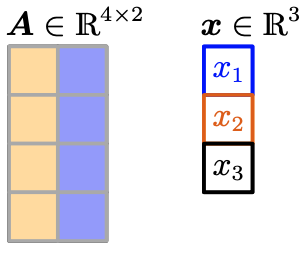
\includegraphics[width=0.9\columnwidth]{L5_grad_matrix_1.png}
}
{
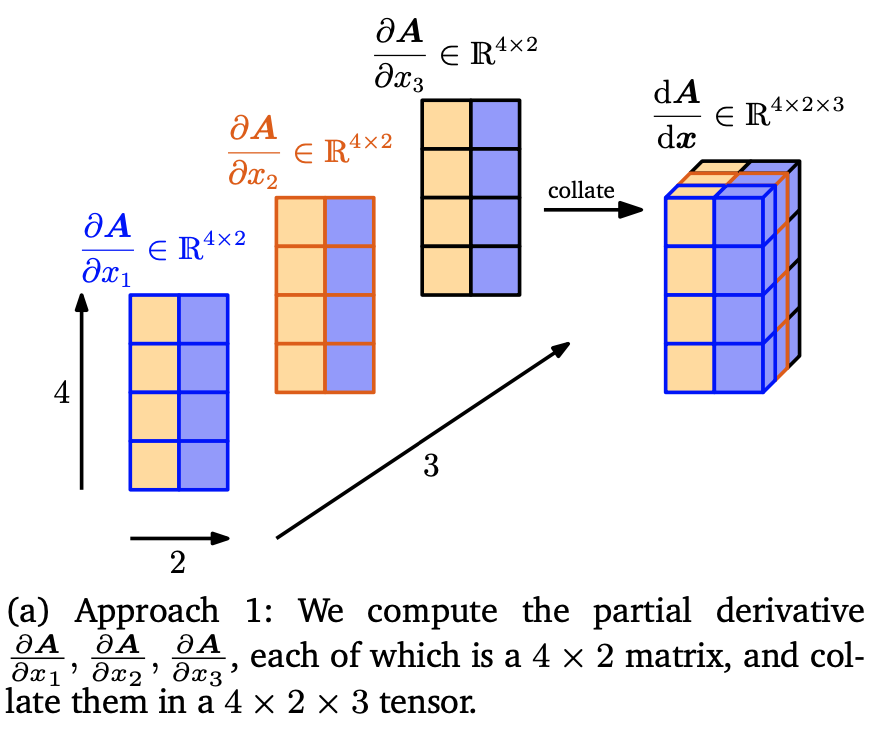
\includegraphics[width=0.47\columnwidth]{L5_grad_matrix_2.png}
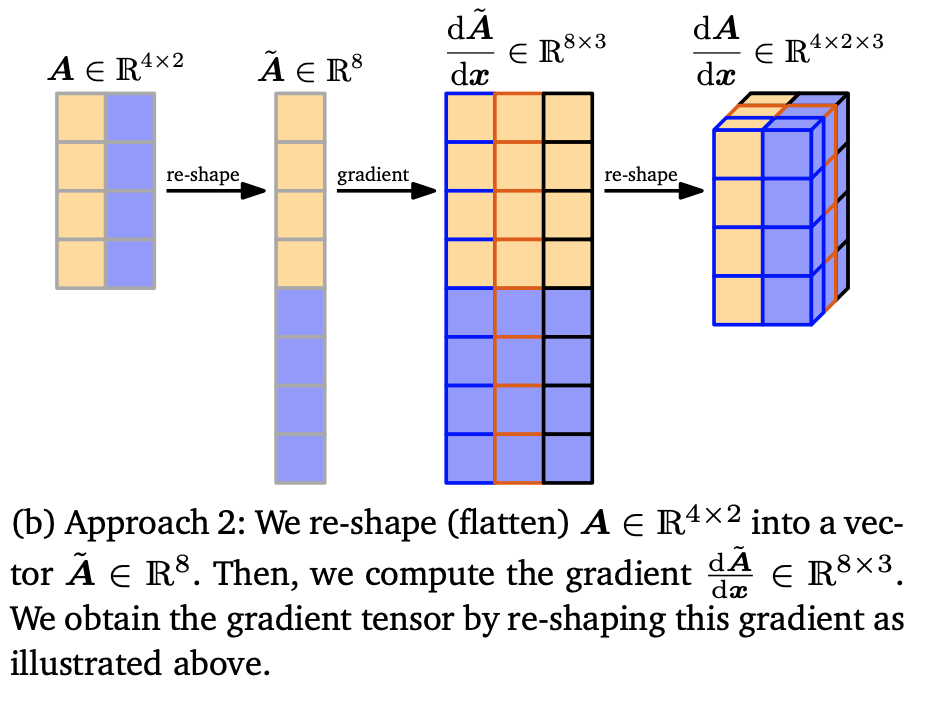
\includegraphics[width=0.47\columnwidth]{L5_grad_matrix_3.png}
}




\end{frame}

%%%%%%%%%%%%%%%%%%%%%%%%%%%%%%%%%%%%%%%%%%%%%%%%%%%%%%
\begin{frame}{Example: Gradient of Vectors for Matrices}

\bci
\item $\vf(\vx) = \mA \vx,$  $\vf \in \realm$, $\mA \in \realmn,$ $\vx \in \realn.$ What is \bluef{$\d{\vf}{\mA}$?}

\item Dimension: If we consider $\vf: \realmn \mapsto \realm,$ $\d{\vf}{\mA} \in \real^{m\times (m \times n)}$


\item Partial derivatives: 
$
 \pd{f_i}{\mA} \in \real^{1\times (m \times n)}, \quad \d{\vf}{\mA} = \colvec{ \pd{f_1}{\mA} \\ \vdots \\  \pd{f_m}{\mA}} 
$
\mytwocols{0.45}
{
\small
\aleq{
f_i &= \sum_{j=1}^n A_{ij} x_j, \ i=1, \ldots, m \implies \pd{f_i}{A_{iq}} = x_q,\cr    
\pd{f_i}{A_{i\cdot}} &= \trans{\vx} \in \real^{1\times 1\times n} \ \text{(for $i$th row vector)}\cr
\pd{f_{i}}{A_{{k\neq i}\cdot}} & = \trans{\vec{0}} \in \real^{1\times 1\times n} \ \text{(for $k$th row vector, $k\neq i$)}
}
}
{
\small
\aleq{
\pd{f_i}{\mA} = \colvec{\trans{\vec{0}} \\ \vdots \\ \trans{\vec{0}} \\ \trans{\vx} \\ \trans{\vec{0}} \\ \vdots \\ \trans{\vec{0}}} \in \real^{1 \times (m \times n)}
}
}

\eci

\end{frame}

%%%%%%%%%%%%%%%%%%%%%%%%%%%%%%%%%%%%%%%%%%%%%%%%%%%%%%
\begin{frame}{Example: Gradient of Matrices for Matrices}

\bci
\item $\mR \in \realmn$ and $\vf: \realmn \mapsto \realnn$ with $\vf(\mR) = \mK \eqdef \trans{\mR}\mR \in \realnn.$  What is \bluef{$\d{\mK}{\mR} \in \real^{(n\times n) \times (m\times n)}$?}

\item $\d{K_{pq}}{\mR} \in \real^{1 \times m \times n}.$ Let $\vr_i$ be the $i$th column of $\mR.$ Then
\(
K_{pq} = \trans{\vr_p} \vr_q = \sum_{k=1}^m R_{kp} R_{kq}.
\)

\item Partial derivative $\pd{K_{pq}}{R_{ij}}$
\aleq{
\pd{K_{pq}}{R_{ij}} = \sum_{k=1}^m \pd{}{R_{ij}} R_{kp} R_{kq} = \partial_{pqij}, \ 
\partial_{pqij} = 
\begin{cases}
R_{iq} & \text{if} \ j=p, p\neq q \cr
R_{ip} &  \text{if} \ j=q, p\neq q \cr
2R_{iq} &  \text{if} \ j=p, p=q \cr
0 & \text{otherwise}
\end{cases}
}
\eci

\end{frame}

%%%%%%%%%%%%%%%%%%%%%%%%%%%%%%%%%%%%%%%%%%%%%%%%%%%%%%
\begin{frame}{Useful Identities}

\vspace{-0.6cm}
\raggedleft
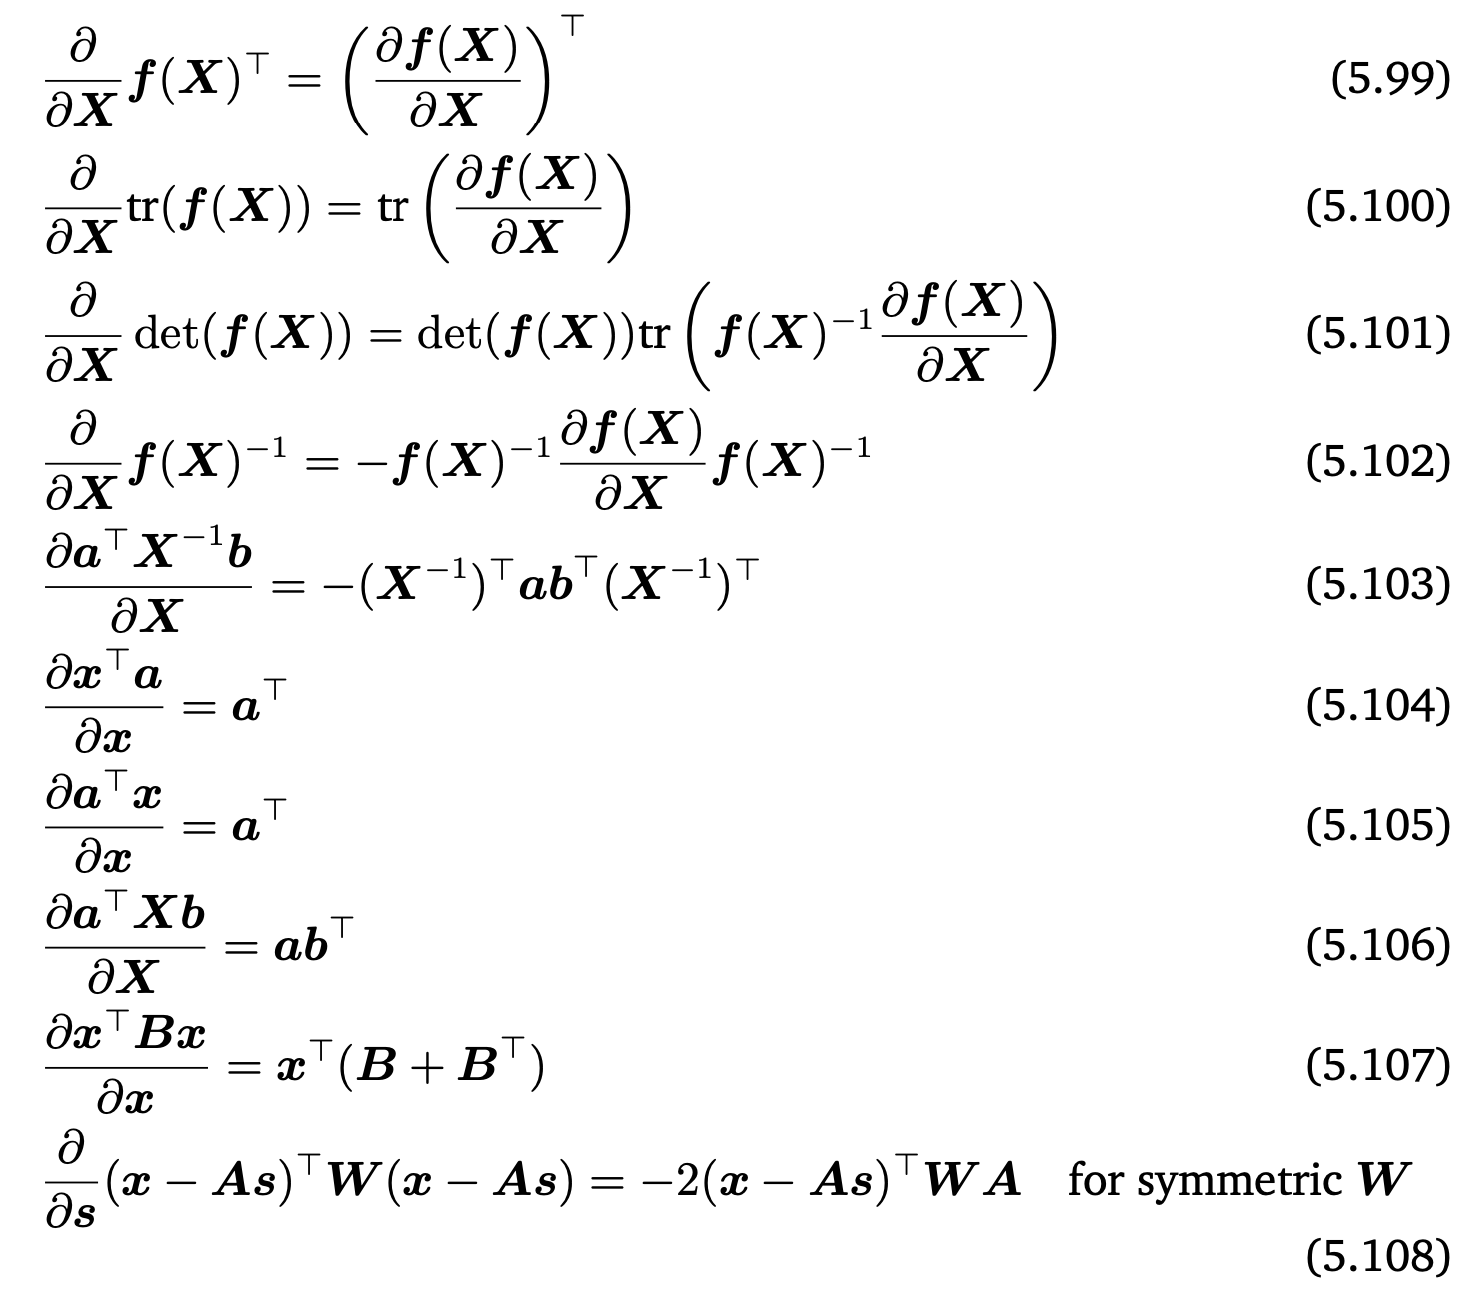
\includegraphics[width=0.7\columnwidth]{L5_useful.png}
\end{frame}


%%%%%%%%%%%%%%%%%%%%%%%%%%%%%%%%%%%%%%%%%%%%%%%%%%%%%%
\begin{frame}{Roadmap}

\plitemsep 0.1in

\bci 
\item \grayf{Differentiation of Univariate Functions}

\item \grayf{Partial Differentiation and Gradients }

\item \grayf{Gradients of Vector-Valued Functions} 

\item \gray{Gradients of Matrices} 

\item \grayf{Useful Identities for Computing Gradients} 

\item \redf{Backpropagation and Automatic Differentiation} 

\item \grayf{Higher-Order Derivatives 

\item Linearization and Multivariate Taylor Series}

\eci
\end{frame}

%%%%%%%%%%%%%%%%%%%%%%%%%%%%%%%%%%%%%%%%%%%%%%%%%%%%%%
\begin{frame}{Motivation: Neural Networks with Many Layers (1)}

\plitemsep 0.01in

\bci 
\item In a neural network with many layers, the function $\vy$ is a many-level function compositions
$$
\vy = (f_K \circ f_{K-1} \circ \cdots \circ f_1)(\vx),
$$
where, for example,  
\bci
\item $\vx$: images as inputs, $\vy$: class labels (e.g., cat or dog) as outputs
\item each $f_i$ has its own parameters
\eci

\item In neural networks, with the model parameters $\vth = \{\mA_0, \vb_0, \ldots, \mA_{K-1}, \vb_{K-1} \}$

\smallskip
\mysmalltwocols{0.4}
{
\small
\vspace{-0.4cm}
\aleq{
\begin{cases}
\vf_0 &\eqdef \vx \cr
\vf_1 &\eqdef \sigma_1(\mA_{0}\vf_{0} + \vb_{0})\cr
\vdots& \cr
\vf_K &\eqdef \sigma_K(\mA_{K-1}\vf_{K-1} + \vb_{K-1})
\end{cases}
}
$\circ$ $\sigma_i$ is called the \bluef{activation function} at $i$-th layer
}
{
\hspace{-0.7cm} $\circ$ Minimizing the loss function over $\vth$:
\aleq{
\min_{\vth} L(\vth),
}
where 
$
L(\vth) = \norm{\vy - \vf_K(\vth,\vx)}^2
$
}

\eci
\end{frame}

%%%%%%%%%%%%%%%%%%%%%%%%%%%%%%%%%%%%%%%%%%%%%%%%%%%%%%
\begin{frame}{Motivation: Neural Networks with Many Layers (2)}

\plitemsep 0.01in

\bci 

\item In neural networks, with the model parameters $\vth = \{\mA_0, \vb_0, \ldots, \mA_{K-1}, \vb_{K-1} \}$

\smallskip
\mysmalltwocols{0.4}
{
\small
\vspace{-0.4cm}
\aleq{
\begin{cases}
\vf_0 &\eqdef \vx \cr
\vf_1 &\eqdef \sigma_1(\mA_{0}\vf_{0} + \vb_{0})\cr
\vdots& \cr
\vf_K &\eqdef \sigma_K(\mA_{K-1}\vf_{K-1} + \vb_{K-1})
\end{cases}
}
$\circ$ $\sigma_i$ is called the activation function at $i$-th layer
}
{
\hspace{-0.7cm} $\circ$ Minimizing the loss function over $\vth$:
\aleq{
\min_{\vth} L(\vth),
}
where 
$
L(\vth) = \norm{\vy - \vf_K(\vth,\vx)}^2
$
}

\medskip
\item \question \bluef{\large How can we efficiently compute $\displaystyle \d{L}{\vth}$ in computers?}

\eci
\end{frame}

%%%%%%%%%%%%%%%%%%%%%%%%%%%%%%%%%%%%%%%%%%%%%%%%%%%%%%
\begin{frame}{Backpropagatin: Example (1)}

\plitemsep 0.1in

\bci 

\item $f(x) = \sqrt{x^2 + \exp(x^2)} + \cos\left (x^2 + \exp(x^2)\right)$



\item Computation graph: Connect via ``elementary'' operations

\smallskip
\mypic{0.7}{L5_computation_graph.png}
\aleq{
\bluef{a} = x^2, \ \bluef{b}=\exp(a), \ \bluef{c}=a+b, \ \bluef{d}=\sqrt{c}, \ \bluef{e}=\cos(c), \ \bluef{f} = d+e
}

\item Automatic Differentiation
\bci
\item  A set of techniques to \bluef{numerically} (not symbolically) evaluate the gradient of a function by working with \bluef{intermediate variables} and applying the \bluef{chain rule}. 
\eci
\eci
\end{frame}

%%%%%%%%%%%%%%%%%%%%%%%%%%%%%%%%%%%%%%%%%%%%%%%%%%%%%%
\begin{frame}{Backpropagation: Example (2)}

\plitemsep 0.1in

\bci 

\item 
% $f(x) = \sqrt{x^2 + \exp(x^2)} + \cos\left (x^2 + \exp(x^2)\right)$
$
\bluef{a} = x^2, \ \bluef{b}=\exp(a), \ \bluef{c}=a+b, \ \bluef{d}=\sqrt{c}, \ \bluef{e}=\cos(c), \ \bluef{f} = d+e
$
\item Derivatives of the intermediate variables with their inputs
\aleq{
\bluef{\pd{a}{x}} = 2x, \ \bluef{\pd{b}{a}}=\exp(a), \ \bluef{\pd{c}{a}}=1 = \bluef{\pd{c}{b}}, \ \bluef{\pd{d}{c}}=\frac{1}{2\sqrt{c}}, \ \bluef{\pd{e}{c}}=-\sin(c), \ \bluef{\pd{f}{d}} = 1 = \bluef{\pd{f}{e}}
}
\item Compute $\displaystyle \pd{f}{x}$ by working backward from the output
\mytwocols{0.3}
{
\small
\vspace{-0.3cm}
\aleq{
\orangef{\pd{f}{c}} &= \bluef{\pd{f}{d}\pd{d}{c}} + \bluef{\pd{f}{e}\pd{e}{c}}, \ \redf{\pd{f}{b}} =\bluef{\pd{f}{c}\pd{c}{b}}  \cr
\greenf{\pd{f}{a}} &= \redf{\pd{f}{b}}\bluef{\pd{b}{a}} + \orangef{\pd{f}{c}}\bluef{\pd{c}{a}}, \ \mybox{$\displaystyle \pd{f}{x}$} =\greenf{\pd{f}{a}}\bluef{\pd{a}{x}}  
}
}
{
\small
\vspace{-0.3cm}
\aleq{
\orangef{\pd{f}{c}} &= 1\cdot \frac{1}{2\sqrt{c}} + 1\cdot (-\sin(c))\cr
\redf{\pd{f}{b}} &= \orangef{\pd{f}{c}} \cdot 1, \quad \greenf{\pd{f}{a}} = \redf{\pd{f}{b}} \exp(a) + \orangef{\pd{f}{c}}\cdot 1 \cr
\mybox{$\displaystyle \pd{f}{x}$} &=\greenf{\pd{f}{a}} \cdot 2x
}
}

\eci
\end{frame}

%%%%%%%%%%%%%%%%%%%%%%%%%%%%%%%%%%%%%%%%%%%%%%%%%%%%%%
\begin{frame}{Backpropagation}

\plitemsep 0.1in

\bci 

\item Implementation of gradients can be very expensive, unless we are careful. 

\item Using the idea of automatic differentiation, the whole gradient computation is decomposed into a set of gradients of elementary functions and application of the chain rule.

\item Why \bluef{backward}? 

\bci
\item In neural networks, the input dimensionality is often much higher than the dimensionality of labels.
\item In this case, the backward computation (than the forward computation) is much cheaper. 
\eci

\item Works if the target is expressed as a computation graph whose elementary functions are differentiable. If not, some care needs to be taken. 
\eci
\end{frame}

%%%%%%%%%%%%%%%%%%%%%%%%%%%%%%%%%%%%%%%%%%%%%%%%%%%%%%
\begin{frame}{Roadmap}

\plitemsep 0.1in

\bci 
\item \grayf{Differentiation of Univariate Functions}

\item \grayf{Partial Differentiation and Gradients }

\item \grayf{Gradients of Vector-Valued Functions} 

\item \gray{Gradients of Matrices} 

\item \grayf{Useful Identities for Computing Gradients} 

\item \grayf{Backpropagation and Automatic Differentiation} 

\item \redf{Higher-Order Derivatives 

\item Linearization and Multivariate Taylor Series}

\eci
\end{frame}

%%%%%%%%%%%%%%%%%%%%%%%%%%%%%%%%%%%%%%%%%%%%%%%%%%%%%%
\begin{frame}{Higher-Order Derivatives}

\plitemsep 0.05in

\bci 
\item Some optimization algorithms (e.g., Newton's method) require second-order derivatives, if they exist. 
\item (Truncated) Taylor series is often used as an approximation of a function. 

\item For $f: \realn \mapsto \real$ of variable $\vx \in \realn$, $
\grad_{\vec{x}} f = \d{f}{\vec{x}} = 
\rowvec{\pd{f(\vec{x})}{x_1} & \cdots & \pd{f(\vec{x})}{x_n}} \in \real^{1 \times n}
$
\bci
\item If $f$ is twice-differentiable, the order doesn't matter. 
\aleq{
\hess_{\vec{x}} f = \begin{nmat}
\pdd{f}{x_1}& \pdda{f}{x_1}{x_2}& \cdots & \pdda{f}{x_1}{x_n}\cr 
\vdots & & & \vdots\cr
\pdda{f}{x_1}{x_n} & \pdda{f}{x_2}{x_n} & \cdots & \pdda{f}{x_{n}}{x_n}
\end{nmat}
}
% Gradient $\grad f: \realn \mapsto $
\eci

\item For $f: \realn \mapsto \realm$, $\grad_{\vec{x}} f \in \realmn$
\bci
\item Thus, $\hess_{\vec{x}} f \in \real^{m \times n \times n}$ (a tensor)
\eci

\eci
\end{frame}

%%%%%%%%%%%%%%%%%%%%%%%%%%%%%%%%%%%%%%%%%%%%%%%%%%%%%%
\begin{frame}{Function Approximation: Lineariation and More}

\plitemsep 0.1in

\bci 
\item First-order approximation of $f(\vx)$ (i.e., linearization by taking the first two terms of Taylor Series)
$$
f(\vx) \approx f(\vx_0) + (\grad_{\vx} f)(\vx_0)(\vx-\vx_0)
$$

\item Multivariate Talyer Series for $f: \real^D \mapsto \real$ at $\vx_0$
$$
f(\vx) = \sum_{k=0}^\infty \frac{D^k_{\vx} f(\vx_0)}{k!} \vec{\delta}^k,
$$
where $D^k_{\vx} f(\vx_0)$ is the $k$th derivative of $f$ w.r.t. $\vx$, evaluated at $\vx_0,$ and $\vec{\delta} \eqdef \vx - \vx_0.$
\bci
\item Partial sum up to, say $n$, can be an approximation of $f(\vx).$
\item $D^k_{\vx} f(\vx_0)$ and $\vec{\delta}^k$ are $k$th order tensors, i.e., $k$-dimensional array. 

\item $\vec{\delta}^k$ is a $k$-fold outer product $\otimes$. For example, $\vec{\delta}^2 = \vec{\delta} \otimes \vec{\delta} = \vec{\delta}\trans{\vec{\delta}}.$ $\vec{\delta}^3 = \vec{\delta} \otimes \vec{\delta} \otimes \vec{\delta}.$ 
\eci

\eci



\end{frame}



%%%%%%%%%%%%%%%%%%%%%%%%%%%%%%%%%%%%%%%%%%%%%%%%%%%%%%
\begin{frame}{}
\vspace{2cm}
\LARGE Questions?


\end{frame}

\begin{frame}{Review Questions}
% \tableofcontents
%\plitemsep 0.1in
\bce[1)]
\item 

\ece
\end{frame}


\end{document}
